\documentclass[12pt,a4paper]{report}

\usepackage{fontspec}
\setmainfont{DejaVu Serif}
\setsansfont{DejaVu Sans}
\setmonofont{DejaVu Sans Mono}
\usepackage[a4paper,margin=2.4cm]{geometry}
\usepackage{setspace}
\onehalfspacing
\usepackage{microtype}
\usepackage{graphicx}
\usepackage{booktabs}
\usepackage{longtable}
\usepackage{array}
\usepackage{tabularx}
\usepackage{enumitem}
\usepackage{xcolor}
\usepackage{listings}
\usepackage{hyperref}
\usepackage{caption}
\usepackage{float}
\usepackage{fancyhdr}
\usepackage{amsmath}
\usepackage{amssymb}
\usepackage{tikz}
\usetikzlibrary{arrows.meta,positioning,shapes.geometric,fit}

\definecolor{codebg}{RGB}{246,248,250}
\definecolor{codeframe}{RGB}{208,215,222}
\definecolor{accent}{RGB}{5,150,105}
\definecolor{datablue}{RGB}{59,130,246}
\hypersetup{
  colorlinks=true,
  linkcolor=accent,
  urlcolor=datablue,
  citecolor=accent,
  pdftitle={Báo cáo kỹ thuật NutriLens AI: Nền tảng AI và dữ liệu dinh dưỡng},
  pdfauthor={Nhóm phát triển NutriLens AI}
}

\lstdefinestyle{nutrilens}{
  backgroundcolor=\color{codebg},
  frame=single,
  rulecolor=\color{codeframe},
  basicstyle=\ttfamily\small,
  breaklines=true,
  columns=fullflexible,
  showstringspaces=false,
  numbers=left,
  numberstyle=\tiny\color{gray},
  xleftmargin=1em,
  framexleftmargin=0.5em
}
\lstset{style=nutrilens}

\pagestyle{fancy}
\fancyhf{}
\fancyhead[L]{NutriLens AI/Data Platform}
\fancyhead[R]{Báo cáo kỹ thuật}
\fancyfoot[C]{\thepage}
\setlength{\headheight}{15pt}

\newcommand{\project}{\textbf{NutriLens AI}}
\newcommand{\code}[1]{\texttt{#1}}
\newcommand{\statusok}{\textcolor{green!50!black}{\textbf{Đã triển khai}}}
\newcommand{\statusroadmap}{\textcolor{orange!80!black}{\textbf{Hướng phát triển}}}

\begin{document}

\begin{titlepage}
  \centering
  \vspace*{1.2cm}
  {\sffamily\bfseries\LARGE BÁO CÁO KỸ THUẬT\par}
  \vspace{0.8cm}
  {\sffamily\bfseries\Huge NUTRILENS AI\\
  NỀN TẢNG AI VÀ DỮ LIỆU DINH DƯỠNG END-TO-END\par}
  \vspace{1.0cm}
  {\Large Hybrid RAG, pgvector, Evaluation Gate và Data Operations\par}
  \vspace{1.5cm}

  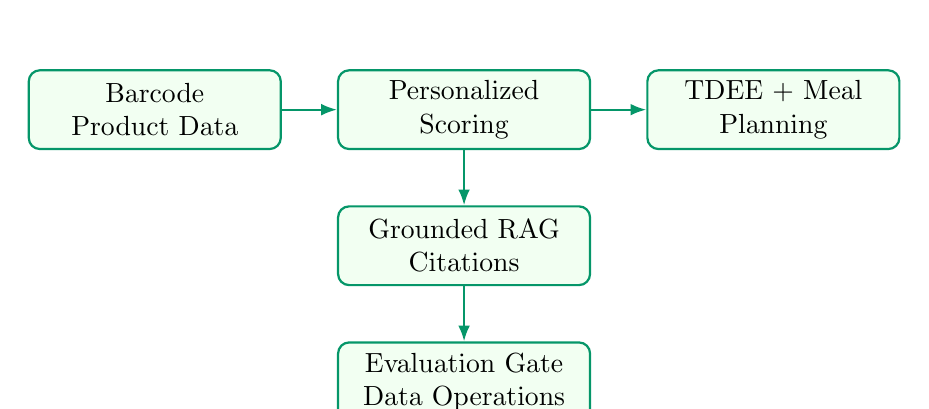
\begin{tikzpicture}[
    node distance=7mm,
    box/.style={draw=accent,rounded corners,align=center,minimum width=3.2cm,
                minimum height=1.0cm,fill=green!5,thick},
    arrow/.style={-{Latex[length=2mm]},thick,draw=accent}
  ]
    \node[box] (scan) {Barcode\\Product Data};
    \node[box,right=of scan] (score) {Personalized\\Scoring};
    \node[box,right=of score] (plan) {TDEE + Meal\\Planning};
    \node[box,below=of score] (rag) {Grounded RAG\\Citations};
    \node[box,below=of rag] (ops) {Evaluation Gate\\Data Operations};
    \draw[arrow] (scan)--(score);
    \draw[arrow] (score)--(plan);
    \draw[arrow] (score)--(rag);
    \draw[arrow] (rag)--(ops);
  \end{tikzpicture}

  \vfill
  \begin{tabular}{rl}
    \textbf{Dự án:} & NutriLens AI\\
    \textbf{Loại tài liệu:} & Báo cáo thiết kế, hiện thực và đánh giá hệ thống\\
    \textbf{Định hướng:} & AI Engineering / Data Engineering\\
    \textbf{Ngôn ngữ:} & Tiếng Việt\\
    \textbf{Ngày cập nhật:} & 11/07/2026\\
  \end{tabular}
  \vfill
  {\large Nhóm phát triển NutriLens AI\par}
\end{titlepage}

\pagenumbering{roman}
\chapter*{Tóm tắt}
\addcontentsline{toc}{chapter}{Tóm tắt}

Báo cáo trình bày thiết kế và hiện thực \project{}, một nền tảng hỗ trợ người
dùng hiểu nhãn thực phẩm, cá nhân hóa quyết định mua sắm, quản lý pantry, tính
TDEE, lập kế hoạch bữa ăn và đặt câu hỏi dinh dưỡng có trích dẫn. Khác với một
ứng dụng chỉ trình diễn giao diện, hệ thống được xây dựng như một dự án
AI/Data Engineering end-to-end với hai data plane độc lập: Product Data và
Knowledge Data.

Product Data lấy từ Open Food Facts, được chuẩn hóa, chấm điểm bằng luật xác
định, cache có TTL và stale fallback. Knowledge Data đi qua metadata validation,
chunking theo heading, embedding, Knowledge Release bất biến, hybrid retrieval
BM25/pgvector và Reciprocal Rank Fusion. Mọi release phải vượt Evaluation Gate
trước khi publish; run thất bại được lưu như dữ liệu vận hành thay vì chỉ tồn
tại trong log.

Phiên bản tại thời điểm báo cáo có 18 tài liệu tri thức, 21 evaluation cases ở
các dataset, 14 SQLAlchemy models, 45 API operations và 42 automated tests.
Frontend Next.js hỗ trợ desktop, mobile PWA và Control Plane quản trị riêng.
Backend FastAPI chạy async với SQLite ở local/test và PostgreSQL 17 + pgvector
ở production. Hệ thống được triển khai theo mô hình Netlify, Render và Neon.

\tableofcontents
\listoffigures
\listoftables
\clearpage
\pagenumbering{arabic}

\chapter{Giới thiệu}

\section{Bối cảnh bài toán}

Nhãn dinh dưỡng chứa nhiều trường có ích nhưng khó diễn giải trong thời gian
ngắn. Người dùng thường cần trả lời đồng thời ba nhóm câu hỏi: sản phẩm chứa gì,
sản phẩm có phù hợp với hồ sơ cá nhân hay không, và một khái niệm dinh dưỡng có
ý nghĩa gì. Một LLM thuần túy có khả năng diễn đạt tốt nhưng không phải nguồn
sự thật cho barcode, calories hay dị ứng. Ngược lại, dữ liệu nhãn thô không đủ
để giải thích bằng ngôn ngữ tự nhiên.

\project{} giải quyết bài toán bằng cách phân chia trách nhiệm:

\begin{quote}
\textbf{Open Food Facts = dữ liệu sản phẩm. Luật xác định = quyết định chấm
điểm. RAG = kiến thức giải thích. Hồ sơ người dùng = ngữ cảnh cá nhân.}
\end{quote}

\section{Mục tiêu}

\begin{enumerate}
  \item Xây dựng workflow scan--score--compare--save--plan hoàn chỉnh.
  \item Giữ product facts tách biệt với dữ liệu sở hữu bởi từng người dùng.
  \item Trả lời câu hỏi dinh dưỡng dựa trên corpus đã duyệt và có citation.
  \item Từ chối trả lời khi retrieval không đủ bằng chứng.
  \item Quản trị corpus bằng release, evaluation, publish và rollback.
  \item Hỗ trợ PostgreSQL FTS + pgvector nhưng vẫn test được bằng SQLite.
  \item Có pipeline lineage, data quality, observability và analytics marts.
  \item Cung cấp trải nghiệm desktop, mobile PWA và admin riêng biệt.
  \item Không biến ước tính dinh dưỡng hoặc TDEE thành chẩn đoán y khoa.
\end{enumerate}

\section{Phạm vi}

Hệ thống tập trung vào dữ liệu nhãn thực phẩm đóng gói và kiến thức dinh dưỡng
tổng quát. NutriLens không chẩn đoán bệnh, không kê chế độ điều trị và không
thay thế chuyên gia. Độ chính xác product facts phụ thuộc mức đầy đủ của Open
Food Facts. Meal plan và TDEE là ước tính hỗ trợ lập kế hoạch.

\chapter{Khảo sát và phân rã miền}

\section{Cấu trúc monorepo}

\begin{longtable}{p{0.27\textwidth}p{0.65\textwidth}}
\toprule
\textbf{Thành phần} & \textbf{Vai trò}\\
\midrule
\endhead
\code{apps/web} & Next.js 16, TypeScript, barcode camera, dashboard, chat, meal planner, mobile PWA và Admin Control Plane.\\
\code{apps/api} & FastAPI, identity, product intelligence, profile/TDEE, personal data, RAG, orchestration và observability.\\
\code{apps/api/data} & Curated Markdown knowledge corpus có metadata và provenance.\\
\code{tests/evaluation} & Dataset JSONL cho routing, grounding, fact coverage, abstention và security.\\
\code{infra/migrations} & Schema PostgreSQL, identity, RAG platform, pgvector và profile TDEE.\\
\code{analytics} & dbt-ready sources, semantic definitions và daily marts.\\
\code{docs} & Architecture, security, data platform, runbook, evaluation và deployment.\\
\bottomrule
\caption{Các thành phần chính của NutriLens}
\end{longtable}

\section{Bounded contexts}

\begin{itemize}
  \item \textbf{Identity}: đăng ký, đăng nhập, demo, JWT, cookie và user resolution.
  \item \textbf{Product Intelligence}: Open Food Facts, normalization, cache, scoring và comparison.
  \item \textbf{Personal Nutrition Data}: profile, TDEE, scans, pantry, favorites và meal plans.
  \item \textbf{Knowledge Corpus}: document, chunk, embedding, release và citation lineage.
  \item \textbf{RAG Evaluation}: benchmark, metrics, slices, confidence interval và gate.
  \item \textbf{Data Operations}: orchestration, quality, artifacts, rollback và analytics.
\end{itemize}

Nguyên tắc quan trọng là product cache được chia sẻ để giảm gọi upstream,
nhưng mọi quyết định cá nhân đều lọc theo \code{user\_id}. Truy vấn tài nguyên
dùng đồng thời resource ID và owner ID để không làm lộ sự tồn tại dữ liệu của
người khác.

\chapter{Kiến trúc hệ thống}

\section{Kiến trúc tổng thể}

\begin{figure}[H]
\centering
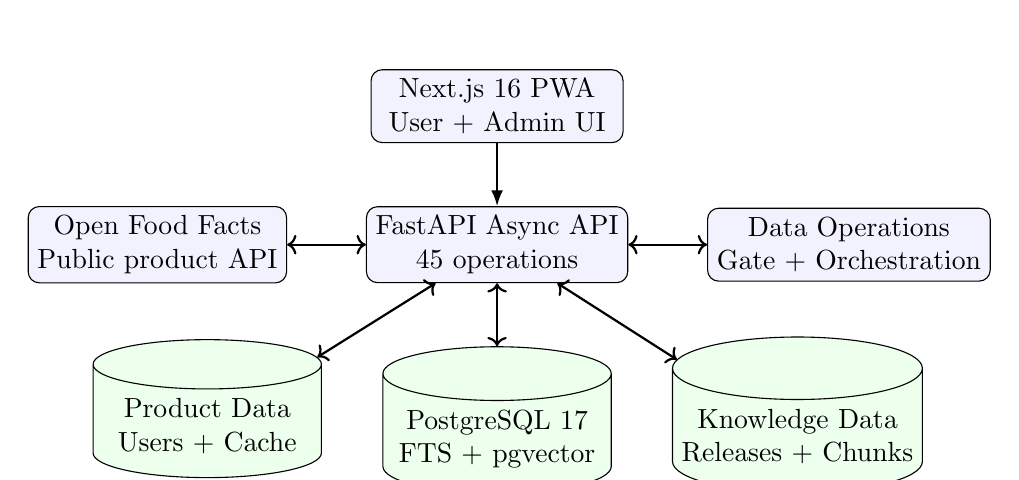
\begin{tikzpicture}[
  node distance=8mm and 10mm,
  box/.style={draw,rounded corners,align=center,minimum width=3.2cm,
              minimum height=0.9cm,fill=blue!5},
  data/.style={draw,shape=cylinder,shape border rotate=90,aspect=0.25,
               align=center,minimum width=2.9cm,minimum height=1.0cm,fill=green!7},
  arrow/.style={-{Latex[length=2mm]},thick}
]
\node[box] (web) {Next.js 16 PWA\\User + Admin UI};
\node[box,below=of web] (api) {FastAPI Async API\\45 operations};
\node[box,left=of api] (off) {Open Food Facts\\Public product API};
\node[box,right=of api] (pipeline) {Data Operations\\Gate + Orchestration};
\node[data,below left=of api] (product) {Product Data\\Users + Cache};
\node[data,below right=of api] (knowledge) {Knowledge Data\\Releases + Chunks};
\node[data,below=of api] (postgres) {PostgreSQL 17\\FTS + pgvector};
\draw[arrow] (web)--(api);
\draw[arrow,<->] (api)--(off);
\draw[arrow,<->] (api)--(pipeline);
\draw[arrow,<->] (api)--(product);
\draw[arrow,<->] (api)--(knowledge);
\draw[arrow,<->] (api)--(postgres);
\end{tikzpicture}
\caption{Kiến trúc logic của NutriLens AI}
\end{figure}

\section{Request lifecycle}

\begin{enumerate}
  \item Middleware tạo hoặc tiếp nhận request ID và bắt đầu đo latency.
  \item Rate limiter phân loại endpoint nhạy cảm.
  \item CORS và JWT cookie xác định caller.
  \item Router gọi domain service và truy vấn owner-scoped.
  \item Response được gắn security headers, request ID và timing.
  \item Chat ghi audit hash, route, abstention, citation count và latency.
\end{enumerate}

\section{Chiến lược lỗi}

Input không hợp lệ trả 422; thiếu xác thực trả 401; tài nguyên không thuộc user
trả 404; upstream lỗi trả stale cache hoặc 502; evidence yếu khiến RAG abstain.
Readiness được tách khỏi startup nặng để container có thể mở port sớm trên nền
tảng free tier.

\chapter{Product Data và cá nhân hóa}

\section{Open Food Facts adapter}

Barcode được validate trước khi gọi upstream. Response được chuẩn hóa về tên,
brand, categories, ingredients, allergens, additives, nutriments, Nutri-Score,
Eco-Score và image. Cache dùng TTL; khi upstream tạm lỗi, record cũ vẫn được
trả để tránh biến sự cố mạng thành outage toàn bộ workflow.

\section{Deterministic scoring}

Scoring engine phân tích calories, sugar, sodium, saturated fat, protein,
fiber, allergens, diet, additives và Nutri-Score. Luật xác định được ưu tiên
trước LLM vì ba lý do: reproducible, dễ test và có thể giải thích field nào đã
làm thay đổi score. Response luôn mang good points, warnings, missing fields và
disclaimer.

\section{TDEE và calorie target}

Hệ thống dùng phương trình Mifflin--St Jeor \cite{mifflin} để ước tính BMR:

\begin{equation}
\mathrm{BMR}=10W+6.25H-5A+S,
\end{equation}

trong đó $W$ là cân nặng kg, $H$ là chiều cao cm, $A$ là tuổi; $S=5$ cho nam
và $S=-161$ cho nữ. TDEE được ước tính bởi:

\begin{equation}
\mathrm{TDEE}=\mathrm{BMR}\times f_{activity}.
\end{equation}

Mục tiêu giảm $L$ kg/tuần tạo deficit yêu cầu $L\times7700/7$ kcal/ngày.
Service giới hạn deficit ở 25\% TDEE và calorie floor tham khảo, đồng thời cảnh
báo khi mục tiêu vượt 1\% cân nặng mỗi tuần. Kết quả được đưa trực tiếp sang
Meal Planner nhưng vẫn được mô tả là ước tính dân số, cần hiệu chỉnh theo theo
dõi thực tế.

\section{Meal planning engine}

Mỗi món có meal type, goals, diets, ingredients, aliases, allergens, kcal,
protein, fiber và estimated cost. Candidate được loại theo diet/dị ứng trước,
sau đó chấm điểm theo mục tiêu, pantry match, lịch sử lặp và budget. Shopping
list được aggregate từ nguyên liệu thật và bỏ các item khớp pantry. Thiết kế
này thay thế bản prototype từng lặp cùng một món cho mọi bữa.

\chapter{Thiết kế Knowledge Data và RAG}

\section{Knowledge corpus}

Corpus tại thời điểm báo cáo gồm 18 tài liệu Markdown về đọc nhãn, sugar,
sodium, protein, fiber, saturated fat, allergens, additives, food safety,
vegetarian/vegan, diabetes, hypertension, children nutrition và các câu hỏi
đời thường như trứng, cá, yogurt--yến mạch, cà phê. Metadata bắt buộc gồm
authority, source URL, jurisdiction, risk level, effective/review dates,
evidence level, domains và status.

\section{Ingestion và immutable release}

\begin{figure}[H]
\centering
\begin{tikzpicture}[
  node distance=6mm,
  box/.style={draw,rounded corners,align=center,minimum width=5.4cm,
              minimum height=0.72cm,fill=gray!6},
  arrow/.style={-{Latex[length=2mm]},thick}
]
\node[box] (source) {Markdown + approved admin documents};
\node[box,below=of source] (validate) {Metadata validation + injection scan};
\node[box,below=of validate] (chunk) {Heading-aware deterministic chunking};
\node[box,below=of chunk] (hash) {Content hash + embedding reuse};
\node[box,below=of hash] (release) {Draft Knowledge Release + manifest};
\node[box,below=of release] (gate) {Evaluation Gate};
\node[box,below=of gate] (publish) {Publish hoặc Blocked};
\draw[arrow] (source)--(validate);
\draw[arrow] (validate)--(chunk);
\draw[arrow] (chunk)--(hash);
\draw[arrow] (hash)--(release);
\draw[arrow] (release)--(gate);
\draw[arrow] (gate)--(publish);
\end{tikzpicture}
\caption{Pipeline tạo Knowledge Release}
\end{figure}

Chunk giữ source filename/title/URL, document ID, heading path, content hash,
token count, metadata, embedding và embedding model. Embedding cũ được reuse
khi cặp \code{content\_hash + embedding\_model} không đổi. Manifest hash làm
release reproducible và hỗ trợ artifact export.

\section{Hybrid retrieval}

Local mode dùng BM25 và feature-hash embedding; production dùng PostgreSQL FTS
và pgvector để lấy candidate. BM25 cho token $t$ trong document $d$:

\begin{equation}
\mathrm{BM25}(t,d)=\mathrm{IDF}(t)\frac{f(t,d)(k_1+1)}
{f(t,d)+k_1(1-b+b\frac{|d|}{\mathrm{avgdl}})}.
\end{equation}

Lexical rank và semantic rank được hợp nhất bằng Reciprocal Rank Fusion:

\begin{equation}
\mathrm{RRF}(d)=\frac{w_l}{k+r_l(d)}+\frac{w_s}{k+r_s(d)}.
\end{equation}

Title và heading được boost. Semantic similarity chỉ refine candidate có
lexical evidence để tránh collision từ feature hashing đưa chunk không liên
quan vào câu trả lời. Alias tiếng Việt hỗ trợ từ có dấu, không dấu và các token
ngắn quan trọng như ``cá'' hoặc ``xơ''.

\section{Answer construction và abstention}

Runtime phân loại route thành RAG, product hoặc mixed. Product-specific facts
không được suy từ corpus. Retrieval hit phải vượt relevance floor; nếu không,
API trả abstained response. Citation chứa source, title, URL, snippet, chunk ID,
heading path, lexical score, semantic score và fused score.

\chapter{Evaluation Gate và Data Operations}

\section{Benchmark}

Repository có 21 JSONL cases, trong đó core benchmark hiện nạp 19 cases từ các
nhóm nutrition, mixed product, abstention, benchmark v2 và everyday food. Hai
case còn lại phục vụ product/security dataset riêng. Mỗi case có thể khai báo
expected route, expected source, required facts và should abstain.

\section{Các metric}

\begin{longtable}{p{0.31\textwidth}p{0.47\textwidth}p{0.14\textwidth}}
\toprule
\textbf{Metric} & \textbf{Ý nghĩa} & \textbf{Gate}\\
\midrule
\endhead
Route accuracy & Tỷ lệ chọn đúng RAG/product/mixed. & $=1.00$\\
Abstain accuracy & Tỷ lệ từ chối đúng khi thiếu evidence. & $=1.00$\\
Source recall & Expected source xuất hiện trong citations. & $\geq0.80$\\
Mean reciprocal rank & Expected source xuất hiện càng sớm càng tốt. & $\geq0.70$\\
Required fact coverage & Tỷ lệ required facts có trong answer. & $\geq0.90$\\
Retrieval latency p95 & Phân vị 95 của retrieval latency. & $\leq250$ ms\\
\bottomrule
\caption{Ngưỡng Evaluation Gate mặc định}
\end{longtable}

Evaluator còn lưu slice metrics, Wilson confidence intervals, retrieval trace
và trend so với run trước. Nếu bất kỳ metric nào vi phạm threshold, release giữ
trạng thái draft và orchestration run chuyển sang blocked.

\section{Orchestration và lineage}

Pipeline chính gồm ingest, evaluation gate và publish. Mỗi stage lưu status,
duration, input/output count, release ID, evaluation run ID và failures. Core
logic không phụ thuộc framework; Prefect là adapter tùy chọn. Cách này cho phép
chạy cùng workflow từ CLI, API admin hoặc orchestrator.

\section{Data quality, observability và analytics}

Quality report theo dõi product completeness, stale ratio, missing fields,
release count, duplicate hashes, empty embeddings và pipeline reliability.
Endpoint \code{/metrics} cung cấp Prometheus exposition. Admin snapshot tổng
hợp citation coverage, abstention, latency và active release. Thư mục
\code{analytics/} chứa dbt-ready marts cho RAG và pipeline theo ngày; semantic
catalog mô tả metric, grain, owner và freshness.

\chapter{Backend, frontend và mobile PWA}

\section{API surface}

\begin{longtable}{p{0.36\textwidth}p{0.54\textwidth}}
\toprule
\textbf{Nhóm endpoint} & \textbf{Chức năng}\\
\midrule
\endhead
\code{/api/auth/*} & Register/signup, login, demo, current session, logout.\\
\code{/api/products/*} & Scan, lookup, deterministic score và comparison.\\
\code{/api/profile} & Profile preferences, body/activity inputs và TDEE.\\
\code{/api/pantry}, \code{/api/favorites} & User-owned shopping and storage workflows.\\
\code{/api/meal-plan/*} & Generate và retrieve personalized meal plans.\\
\code{/api/chat/stream} & Grounded answer, route, citations và retrieval trace.\\
\code{/api/rag/search} & Retrieval debugging có score breakdown.\\
\code{/api/admin/*} & Documents, releases, gate, rollback, pipeline, quality và marts.\\
\code{/health/*}, \code{/metrics} & Container health và observability.\\
\bottomrule
\caption{Các nhóm API chính}
\end{longtable}

\section{Identity và security}

Password được hash bằng Argon2; access token dùng JWT trong HttpOnly cookie.
Production yêu cầu secret mạnh, secure cookie và CORS origin giới hạn. Admin
operation yêu cầu \code{X-Admin-Key}. Raw prompt không được lưu; audit chỉ giữ
hash một chiều. Prompt-injection patterns được kiểm tra khi ingest admin
document. Response dùng CSP, frame denial, content-type protection và request
ID.

\section{Frontend và mobile}

Next.js App Router cung cấp dashboard, scanner, product detail, compare, chat,
pantry, favorites, meal planner, profile và admin. Mobile UI có sticky header,
bottom navigation, bottom sheet, safe-area cho iOS, touch target, camera viewport
ổn định và kiểm tra horizontal overflow ở viewport 390x844. Manifest hỗ trợ
standalone PWA và shortcuts cho scan, chat, meal planner.

\chapter{Kiểm thử và kết quả}

\section{Chiến lược kiểm thử}

\begin{table}[H]
\centering
\begin{tabularx}{\textwidth}{lX}
\toprule
\textbf{Nhóm} & \textbf{Nội dung}\\
\midrule
Auth integration & Cookie lifecycle, demo, admin access và cross-user isolation.\\
Product data & Cache freshness, timezone, stale fallback và upstream failure.\\
Scoring & Sugar, diet, allergen và missing-data behavior.\\
Meal/TDEE & Diversity, vegan/exclusion, budget, calorie guardrail và công thức BMR.\\
RAG core & Tokenization, embedding, BM25/RRF, citations và abstention.\\
Data platform & Release lineage, reuse, gate, rollback, orchestration, quality và artifacts.\\
Frontend & ESLint, TypeScript, Next.js production build.\\
Browser E2E & Authenticated portfolio flow và mobile navigation/overflow.\\
\bottomrule
\end{tabularx}
\caption{Phạm vi kiểm thử tự động}
\end{table}

\section{Kết quả kiểm chứng}

Tại thời điểm lập báo cáo:

\begin{itemize}
  \item 42/42 Python tests vượt qua;
  \item Ruff API lint vượt qua;
  \item ESLint không có error (còn một warning font từ Next.js);
  \item Next.js 16 production build thành công với 12 routes;
  \item 2/2 mobile E2E tests vượt qua ở viewport 390x844;
  \item Evaluation Gate thử nghiệm với corpus mở rộng đã publish thành công;
  \item một run kiểm chứng đạt source recall 0.8824, MRR 0.7353 và required
  fact coverage 0.9688, đều vượt threshold tương ứng.
\end{itemize}

Các metric cuối là kết quả của một evaluation run cụ thể, không phải hằng số
được hard-code. Mỗi thay đổi corpus/retrieval phải tạo run mới và đi qua gate.

\section{Các regression tiêu biểu}

\begin{enumerate}
  \item Meal planner ban đầu dùng một pool nhỏ nên lặp yogurt cho nhiều bữa;
  được thay bằng catalog có slot, macro, ingredient và diversity penalty.
  \item Vegan đồng thời tránh soy làm hết candidate bữa sáng; test phát hiện và
  catalog được bổ sung lựa chọn oats/chia không soy.
  \item Feature-hash semantic collision đưa đoạn trứng/cà phê vào câu protein;
  semantic rank được giới hạn trong lexical-grounded candidates.
  \item Tokenizer bỏ từ ngắn dưới ba ký tự, làm mất ``cá'' và ``xơ''; alias-aware
  token retention giúp Evaluation Gate tăng source recall.
  \item PostgreSQL không chấp nhận phép toán giữa datetime aware/naive trong
  product cache; timestamp contract được chuẩn hóa cho asyncpg.
  \item Container từng bị health check trước khi mở port; schema initialization
  được đưa ra background và health endpoint hỗ trợ preflight.
\end{enumerate}

\chapter{Triển khai và vận hành}

\section{Mô hình triển khai}

\begin{table}[H]
\centering
\begin{tabularx}{\textwidth}{lXX}
\toprule
\textbf{Thành phần} & \textbf{Nền tảng} & \textbf{Vai trò}\\
\midrule
Frontend & Netlify & Next.js PWA, redirects cùng origin tới API.\\
Backend & Render & Root Dockerfile, Uvicorn, health/readiness.\\
Database & Neon & Managed PostgreSQL, SSL pooler và pgvector.\\
\bottomrule
\end{tabularx}
\caption{Production deployment hiện tại}
\end{table}

\section{Khởi động local}

\begin{lstlisting}[language=bash]
python -m venv .venv
source .venv/bin/activate
pip install -r apps/api/requirements.txt
npm ci

npm run dev:api
# terminal thu hai
npm run dev:web
\end{lstlisting}

Full stack PostgreSQL:

\begin{lstlisting}[language=bash]
docker compose up --build
curl http://localhost:8000/health/ready
curl http://localhost:8000/metrics
\end{lstlisting}

\section{Data operations}

\begin{lstlisting}[language=bash]
npm run data:pipeline
npm run data:evaluate
npm run data:quality
npm run data:analytics
npm run data:search -- "An trung co tot khong?"
npm run validate
npm run test:e2e
\end{lstlisting}

Sau deploy corpus mới, operator phải chạy release pipeline ở Admin Control
Plane. Runtime tiếp tục dùng published release cũ cho đến khi candidate mới
vượt gate; đây là hành vi có chủ đích.

\chapter{Bảo mật, đạo đức và giới hạn}

\section{Threat model}

Các rủi ro gồm prompt injection, poisoned document, cross-user data access,
secret exposure, insecure cookie, upstream data sai/thiếu, overconfident health
answer và abuse admin endpoint.

\begin{longtable}{p{0.34\textwidth}p{0.54\textwidth}}
\toprule
\textbf{Kiểm soát} & \textbf{Hiện thực}\\
\midrule
\endhead
Identity & Argon2, JWT, HttpOnly/Secure cookie, active-user check.\\
Ownership & Mọi personal resource query dùng \code{user\_id}.\\
Admin boundary & Control Plane riêng và \code{X-Admin-Key}.\\
Prompt privacy & SHA-256 question hash; không lưu raw question trong audit.\\
Corpus safety & Metadata validation, injection scan, approved status.\\
Grounding & Citation lineage, lexical evidence gate và abstention.\\
Operational security & CORS allowlist, rate limit, security headers, request ID.\\
Release safety & Evaluation Gate không bypass, immutable release và rollback.\\
\bottomrule
\caption{Các kiểm soát bảo mật chính}
\end{longtable}

\section{Giới hạn}

Open Food Facts là dữ liệu cộng đồng nên có thể thiếu hoặc sai. Feature hashing
phù hợp reproducible test nhưng không thay thế neural embedding ở quy mô lớn.
Corpus 18 tài liệu và core benchmark 19 cases vẫn nhỏ so với production health
assistant. TDEE, deficit và meal-plan macro là ước tính. Hệ thống không phù hợp
để chẩn đoán, điều trị hoặc xử lý emergency.

\chapter{Hướng phát triển}

\begin{enumerate}
  \item Mở rộng benchmark lên hàng trăm câu, thêm adversarial và multilingual slices.
  \item Thử nghiệm sentence-transformer tiếng Việt và reranker cross-encoder.
  \item Thêm offline/online retrieval evaluation và A/B experiment registry.
  \item Dùng Alembic cho migration lifecycle thay vì chỉ bootstrap idempotent.
  \item Triển khai dbt warehouse, freshness test và data contract CI.
  \item Thêm object storage cho artifacts và retention policy.
  \item Thêm alert dashboard cho gate failure, latency và citation coverage.
  \item Mở rộng meal catalog, serving scaling và optimizer theo macro constraints.
  \item Hiệu chỉnh TDEE bằng chuỗi cân nặng quan sát được với privacy controls.
  \item Bổ sung nguồn hướng dẫn dinh dưỡng chính thống theo jurisdiction Việt Nam.
\end{enumerate}

\chapter{Kết luận}

\project{} chứng minh một ứng dụng AI đáng tin cậy cần nhiều hơn một chat box.
Giá trị cốt lõi nằm ở data contracts, deterministic domain logic, retrieval có
lineage, evaluation gate, pipeline observability và failure behavior rõ ràng.
Việc tách Product Data khỏi Knowledge Data cho phép hệ thống vừa phản hồi dữ
liệu barcode cụ thể, vừa giải thích kiến thức có nguồn mà không trộn hai loại
sự thật.

Kiến trúc hiện tại đủ để trình diễn năng lực end-to-end của AI/Data Engineer:
ingestion, normalization, storage, retrieval, evaluation, orchestration,
analytics, API, frontend và deployment. Đồng thời, các disclaimer và abstention
giữ phạm vi của sản phẩm ở mức hỗ trợ thông tin thay vì tạo cảm giác chẩn đoán
y khoa.

\appendix
\chapter{Ví dụ truy vấn đánh giá}

\begin{longtable}{p{0.48\textwidth}p{0.42\textwidth}}
\toprule
\textbf{Câu hỏi} & \textbf{Nguồn/route mong đợi}\\
\midrule
\endhead
Ăn trứng có tốt không? & \code{eggs\_and\_health.md}, RAG.\\
Uống cà phê mỗi ngày có sao không? & \code{coffee\_and\_caffeine.md}, RAG.\\
Yogurt và yến mạch có phù hợp cho bữa sáng? & Breakfast guidance, RAG.\\
Tôi dị ứng sữa, sản phẩm này dùng được không? & Food allergens, mixed.\\
Protein trên nhãn dinh dưỡng có ý nghĩa gì? & Protein basics, RAG.\\
Một chất bí mật XZ-991 chữa bệnh gì? & Abstain.\\
\bottomrule
\caption{Các câu hỏi regression đại diện}
\end{longtable}

\chapter{API mẫu}

\begin{lstlisting}[language=bash]
curl -X POST http://localhost:8000/api/products/scan \
  -H 'Content-Type: application/json' \
  -d '{"barcode":"737628064502"}'

curl -X POST http://localhost:8000/api/chat/stream \
  -H 'Content-Type: application/json' \
  -d '{"question":"An trung co tot khong?","barcode":null}'

curl -X POST http://localhost:8000/api/profile/tdee \
  -H 'Content-Type: application/json' \
  -d '{"biological_sex":"male","age":30,"height_cm":175,
       "weight_kg":75,"activity_level":"moderate",
       "target_weight_loss_kg_week":0.5,"goal":"weight_loss"}'
\end{lstlisting}

\begin{thebibliography}{99}
\bibitem{off}
Open Food Facts, \emph{Open Food Facts API Documentation}.
\url{https://openfoodfacts.github.io/openfoodfacts-server/api/}.

\bibitem{mifflin}
M. D. Mifflin et al., \emph{A New Predictive Equation for Resting Energy
Expenditure in Healthy Individuals}, American Journal of Clinical Nutrition,
51(2), 1990. \url{https://pubmed.ncbi.nlm.nih.gov/2305711/}.

\bibitem{rag}
P. Lewis et al., \emph{Retrieval-Augmented Generation for Knowledge-Intensive
NLP Tasks}, NeurIPS, 2020. \url{https://arxiv.org/abs/2005.11401}.

\bibitem{rrf}
G. V. Cormack, C. L. A. Clarke, S. Buettcher, \emph{Reciprocal Rank Fusion
Outperforms Condorcet and Individual Rank Learning Methods}, SIGIR, 2009.

\bibitem{pgvector}
pgvector, \emph{Open-source Vector Similarity Search for Postgres}.
\url{https://github.com/pgvector/pgvector}.

\bibitem{owasp}
OWASP Foundation, \emph{OWASP Top 10 for Large Language Model Applications}.
\url{https://genai.owasp.org/llm-top-10/}.

\bibitem{niddk}
National Institute of Diabetes and Digestive and Kidney Diseases,
\emph{Body Weight Planner}. \url{https://www.niddk.nih.gov/bwp}.
\end{thebibliography}

\end{document}
